\documentclass[a4paper, twoside]{article}

\usepackage[font={small,it}]{caption}
\usepackage{graphicx}
\usepackage{wrapfig}

\setlength{\oddsidemargin}{0in} \setlength{\evensidemargin}{0in}
\setlength{\textwidth}{6.2in}
\setlength{\topmargin}{-0.3in} \setlength{\textheight}{9.8in}

\title{CS25710 - Travel Trouble}
\author{Tom Leaman (thl5)}

\begin{document}
\maketitle
\newpage
%\tableofcontents
%\newpage

\section{Hardware}

\subsection{Components}

\subsubsection{Microcontroller}
\begin{wrapfigure}[9]{l}{0.25\textwidth}
	\vspace{-18pt}
	\begin{center}
		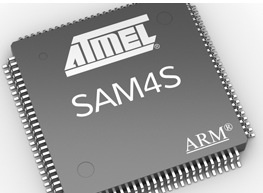
\includegraphics[scale=0.25]{images/atmel_sam4sd32.jpg}
	\end{center}
	\caption{Atmel SAM4SD32B}
\end{wrapfigure}

I began by looking at boards specifically designed for prototyping mobile and
embedded devices, such as the Arduino. These devices are typically very well supported,
often with a strong community of enthusiastic and knowledgeable users. I decided against
actually using an Arduino or similar, however, as they are typically slightly
bulkier and more power-hungry than simpler, more bespoke alternatives.

In the end, I have specified an Atmel SAM4SD32B. This microcontroller can run at
a lower voltage (1.62 - 3.6v) and is small enough to be attached to the
inside of even the smallest suitcase without too much hinderance to the case's
primary function of storing one's luggage!

The SAM4SD32B is equipped with 47 general I/O pins, an A/D converter, a
Synchronous Serial Controller and USB and SD connections. The microcontroller is
also capable of running in a number of low-power modes which will be a necessity
in keeping the device's power consumption to a minimum during its operational
life.

\subsubsection{Accelerometer/Gyro}
\begin{wrapfigure}{r}{0.25\textwidth}
	\begin{center}
		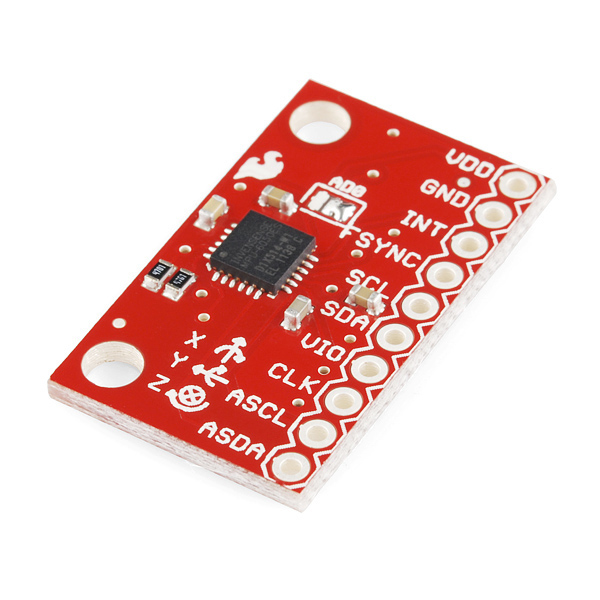
\includegraphics[scale=0.3]{images/mpu-6050.jpg}
	\end{center}
	\caption{InvenSense MPU-6050}
\end{wrapfigure}

I have selected a combined Accelerometer-Gyro, the MPU-6050. This is a 3-axis
Accelerometer and Gyro built into a single board. The device is capable of
measuring movement within a range of programmatically selected ranges which may
allow the client to record a range of movement events during the device's
deployment.

I intend to make use of the accelerometer's available interrupt routines to
wake-up the microcontroller when movement is occurring. I am intending to
collect data approximately every 0.5 seconds during 'gentle' movement (such as
might occur when walking around with the case). I intend to capture data far
more rapidly during 'shock' events, I believe capturing around 1000 times per
second (for half a second or so) should be adequate.

I did consider using a separate accelerometer and gyro but these typically will
not only take more physical space and power but also, many of the 3-axis gyros I
found were actually more expensive on their own than the combined IMU specified
above.

\subsubsection{GPS}
\begin{wrapfigure}{l}{0.25\textwidth}
	\vspace{-35pt}
	\begin{center}
		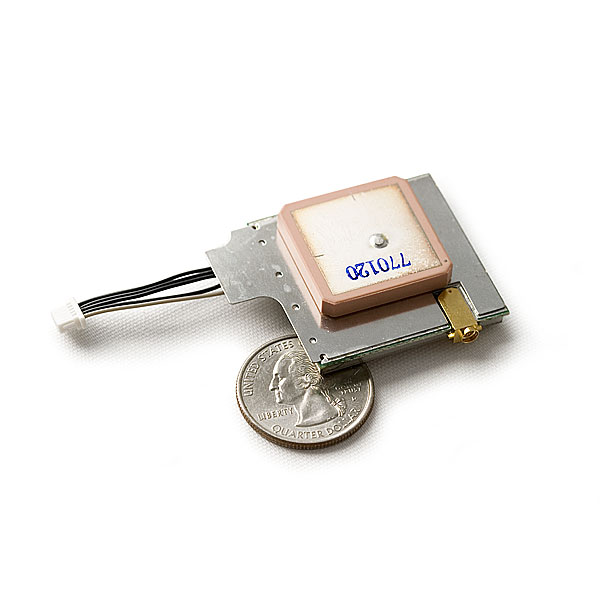
\includegraphics[scale=0.2]{images/em-408.jpg}
	\end{center}
	\vspace{-20pt}
	\caption{GlobalSat EM-408}
\end{wrapfigure}

When selecting a GPS, I tried to find one with a good signal strength (it will
likely be subject to a few layers of various materials which may hamper its
ability to communicate with the necessary satellites. I also tried to find
devices with an on-board antenna as this will reduce the overall form factor.

In the end, I have specified the EM-408. This is capable of 10m accuracy (which
I anticipate will be more than enough for this application), and a high degree of
sensitivity (-159dBm). The EM-408 is capable of outputting data in a number of
well supported formats and more consultation would be required with the client
to ascertain exactly what data they require for their analysis.

\clearpage
\subsubsection{Temperature}
\begin{wrapfigure}{r}{0.25\textwidth}
	\vspace{-40pt}
	\begin{center}
		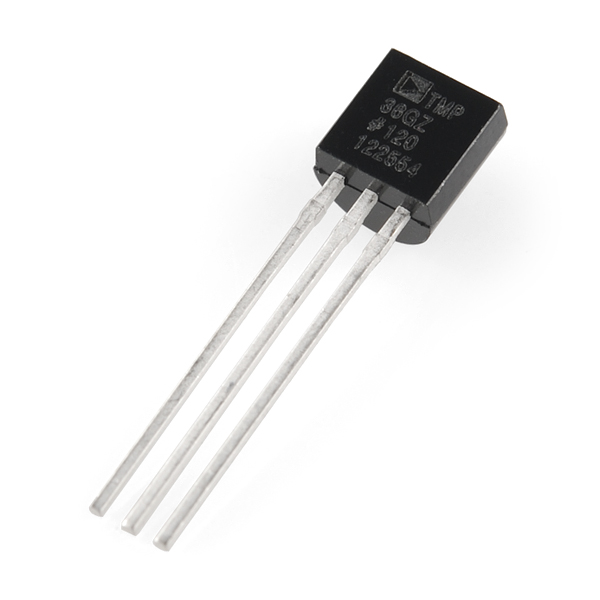
\includegraphics[scale=0.4]{images/tmp36.jpg}
	\end{center}
	\caption{Analog Devices TMP36}
\end{wrapfigure}

I have specified the use of a TMP36 temperature sensor. This is a very small,
low-powered component which can measure temperature accurate to within 1 or 2
degrees (accuracy is reduced at higher temperatures).

\subsubsection{Cells}
\begin{wrapfigure}{l}{0.25\textwidth}
	\vspace{-20pt}
	\begin{center}
		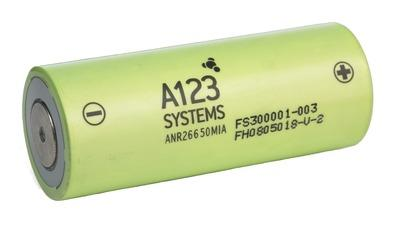
\includegraphics[scale=0.15]{images/a123.jpg}
	\end{center}
	\caption{OSN Power Tech A123}
	\vspace{-20pt}
\end{wrapfigure}

I have calculated that the device will draw around 130mA when capturing data and
around 0.2mA in standby mode. I am assuming the device will be in capture mode
for approx 5\% of its operation. This works out at 2247.84mAh during the
device's two-week operation.

I have decided to specify a Lithium Ion battery. This has a very low rate of
self discharge and should provide a reasonable stable power supply during
operation. These cells also have the added benefit of being rechargeable and
should last for around 2000 uses if cared for properly.

I have decided to specify the use of 1 A123 (ANR26650M1B) cell. This cell will output
3.3v at up to 150A (capacity 2500mAh. Unfortunately, I have only been able to
locate 1 supplier for this exact model of cell which requires a minimum order of
50 pieces. I would be keen to discuss alternative power configurations with the
client, but I believe this cell to be the most ideal for the task at hand.

\subsubsection{Extra components}
I would like to add a single LED indicator which will be switched on when the
device is capturing data (i.e. when it's moving). This will enable the user to
quickly ascertain whether the device is working or not by simply moving the
device (thus triggering the accelerometer) and seeing whether the LED lights up
or not.

\subsection{Major alternatives}
Aside from using an Arduino as the base for the project (outlined above),
another option would be to use a smartphone with an open, extensible software
platform included (for example, and Android phone). These devices typically have
many of the sensory devices required to achieve the necessary functionality
(with the omission, perhaps, of temperature sensing). I believe this would
significantly reduce the overall cost and development time.

I believe the main drawback of this approach is that the device would not be as
flexible in terms of component selection (it would be a much larger operation
to, for example, install a different GPS sensor) and the components it contains
may not be able to sense accurately or fast enough to capture the level of data
required to be useful to the client.

\subsection{Data storage}
I intend to make use of an SD card to hold the data captured by the device.
These are very compact and reasonably priced storage media and will allow the
client to simply transfer the card into their own machine to interpret and
analyse the data. In addition to this, the microcontroller has 2MB of flash
memory built-in which I intend to use as a write cache before the data gets sent
to the SD card. This should avoid a bottle-neck of data trying to be written to
disk during shock events.

In addition to the accelerometer and gyro information being captured (outlined
above), I intend to capture GPS and temperature data around once every 5mins while the device is
moving.

\clearpage
\subsection{Connection diagram}
\begin{center}
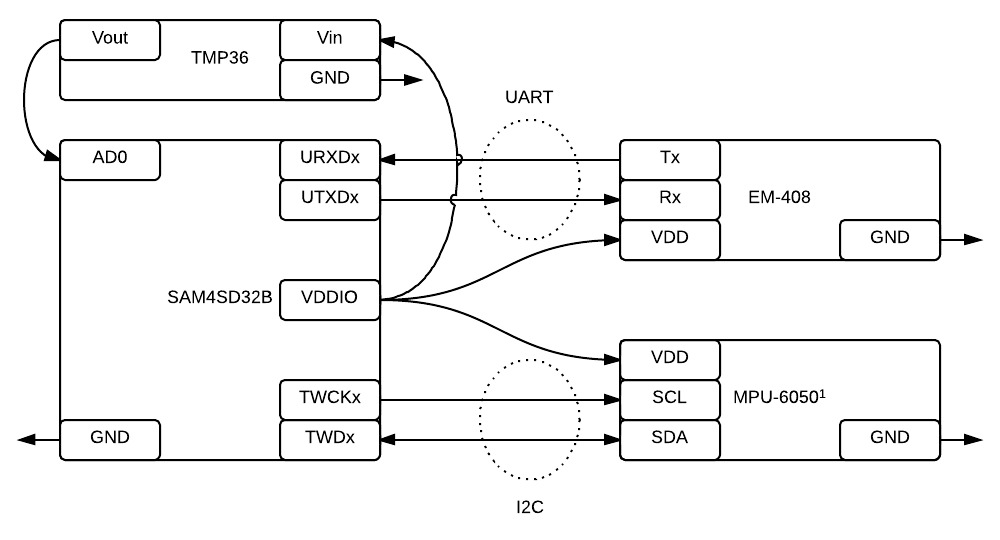
\includegraphics[scale=0.45]{images/connectiondiagram.jpeg}
\end{center}
\footnotetext[1]{I believe the MPU-6050 will also require the VLOGIC and INT pins to be
connected to the microcontroller to enable the microcontroller to wake from
sleep mode when movement commences. I have not been able to ascertain from the
datasheets available where these connections should be made, however. I believe
that the connections are available on the microcontroller though and someone
with more experience than myself should not have a problem locating the correct
connections.}

\subsection{Power consumption}

\begin{tabular}{|l|r|r|}
	\hline
	\textbf{Device} & \textbf{Active state} & \textbf{Idle state} \\
	\hline
	\hline
	SAM4SD32B & 80mA & 32$\mu$A \\
	MPU-6050 & 4.1mA & 115$\mu$A \\
	EM-408 & 44mA & N/A \\
	TMP36 & 50$\mu$A & 0.5$\mu$A \\
	\hline
	\hline
	Total & 128.15mA & 147.5$\mu$A \\
	\hline
\end{tabular}
\vspace{20pt}

All devices will run at 3.3v. It may be necessary to regulate the voltage from
the cells as the actual output voltage is likely to change throughout their
discharge cycle but for the sake of brevity, this has not been included in this
design; it should be trivial to add one at a later date as needed.

\clearpage
\subsection{Dimensions}
\begin{center}
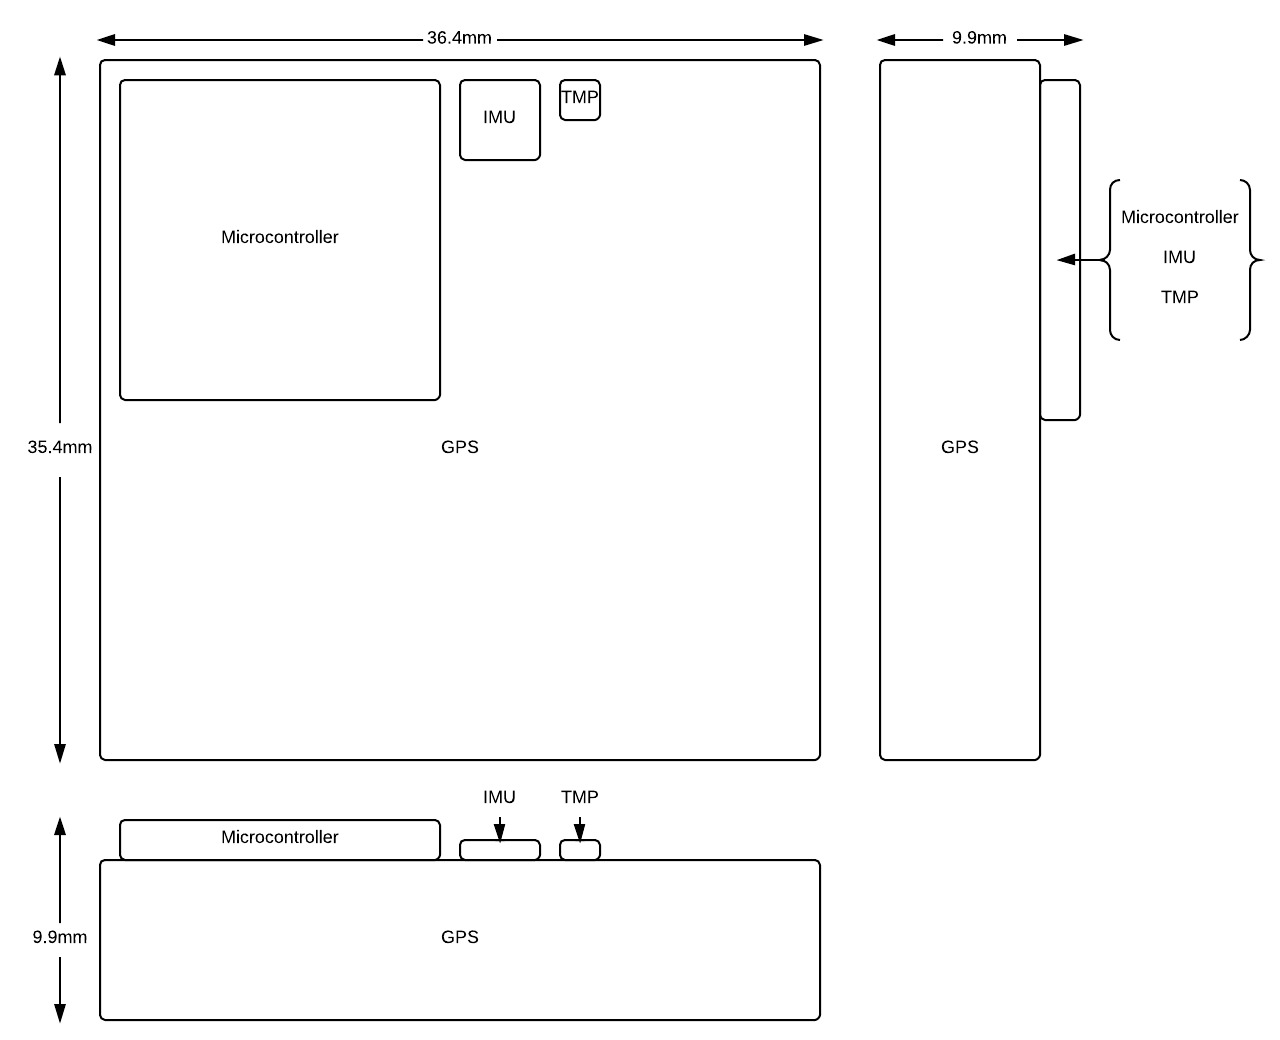
\includegraphics[scale=0.25]{images/layout.jpeg}
\end{center}

The diagram above shows one possible configuration of the devices (albeit
without the cell). This configuration maintains the smallest dimensions for the
device overall. I would recommend mounting the entire unit inside of a plastic
case with battery holder (these are easily available and relatively cheap).

\subsubsection{Weight}
\begin{tabular}{|l|r|}
	\hline
	\textbf{Device} & \textbf{Weight} \\
	\hline
	\hline
	SAM4SD32B & 0.8g \\
	MPU-6050 & $\textless$0.01g \\
	EM-408 & 20g \\
	TMP36 & 5.7g \\
	A123 & 72.5g \\
	\hline
	\hline
	Total & 99g \\
	\hline
\end{tabular}

\subsection{Bill of materials}

\begin{tabular}{|l|r|r|}
	\hline
	\textbf{Device} & \textbf{Single unit} & \textbf{100 units} \\
	\hline
	\hline
	SAM4SD32B\footnotemark[2] & \pounds96.53 & \pounds96.53 \\
	MPU-6050 & \pounds13.09 & \pounds10.47 \\
	EM-408 & \pounds42.63 & \pounds34.10 \\
	TMP36 & \pounds0.98 & \pounds0.79 \\
	A123\footnotemark[3] & N/A & Unknown \\
	\hline
	\hline
	Total & \pounds153.23 & \pounds141.79 \\
	\hline
\end{tabular}
\footnotetext[2]{This price is based on the SAM4S-EK2 'Evaluation Kit' which
contains many extra components used in development of which only 1 or 2 should
ever need to be purchased. Your mileage may vary.}
\footnotetext[3]{I was completely unable to locate
an actual price for the cells online so this has not been
included in the calculation.}

\clearpage
\section{Software}

\subsection{Block diagram}
\begin{center}
	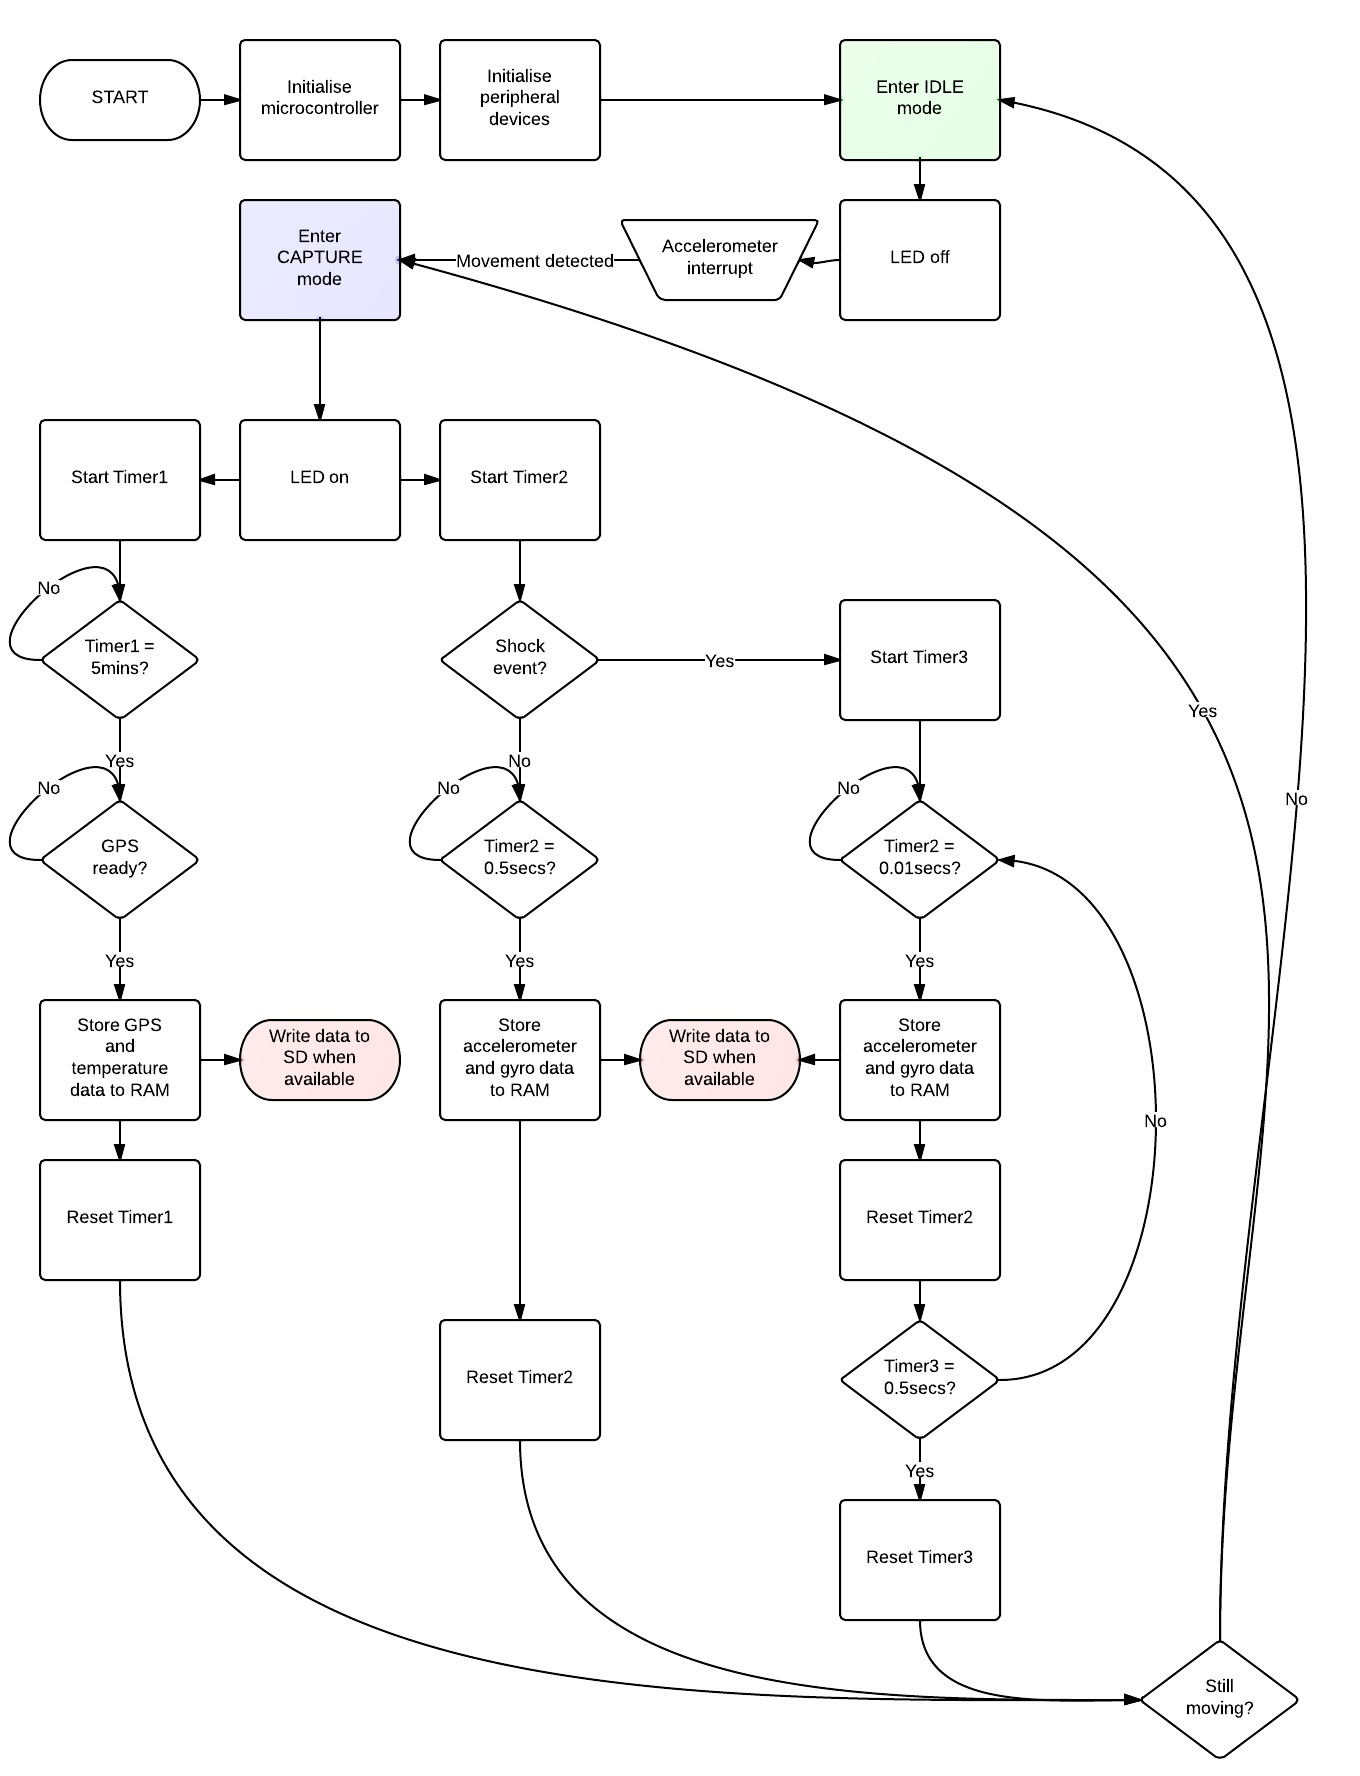
\includegraphics[scale=0.35]{images/software.jpeg}
\end{center}

\subsection{Detailed description}
The software breaks down into 4 main sections:

\subsubsection{Initialisation/Idle}
When the device first receives power, it will initialise all the devices,
including the accelerometer interrupt, and put them into low-power mode. I
anticipate the device will spend the majority of the time in this state,
awaiting sensory input.

\subsubsection{Capture state}
When movement is detected by the IMU, the device will enter a capture mode which
will capture accelerometer/gyro data every 0.5 seconds. This also starts the GPS
routine outlined below. If the force recorded by the accelerometer is great
enough, however, the system will switch to Shock state.

\subsubsection{Shock state}
This state is triggered by excessive, sudden movement being recorded by the
accelerometer. This state will start by setting a timer to control the total
time spent in this state (0.5 seconds) and will capture data at a higher rate
(every 0.001 seconds) until the 0.5 seconds have elapsed.

\subsubsection{GPS}
In addition to the Capture state outlined above, the device will start another
timer when movement is detected. This timer will time a 5minute interval after
which GPS and temperature data will be captured.

\subsubsection{Other considerations}
Attention should be paid to the situations where the device actually writes data
to the SD card (marked on the diagram in red). As stated previously, the
intention is to use the memory on-board the microcontroller as a write cache and
the intention here is to (hopefully) start some subroutine which may handle the
writing of the data to the SD card in parallel to the remainder of the
operations the device is undertaking to perform during capture states.

It should be noted also that I feel the exact details of how the software moves
from capturing data back into an idle state may prove to not be the most
efficient use of the low-power modes available; that is, currently, when the
device is in Capture mode (recording data every 0.5 seconds), there is no
provision for moving into the Idle state if the case is still moving.

\subsection{Development plan}
The microcontroller's manufacturers (Atmel) provide an IDE specifically for
working with this range of devices which I would recommend using. This will,
obviously, require a PC capable of running the software in addition to a USB
connection to transfer the program onto the board.

I would recommend concentrating on successfully gathering data from the IMU
(including registering the interrupts required) as without this, the device will
not get past the Idle state. I would then work incrementally, using the diagram
above as a template (working from top to bottom and right to left) to implement
the remaining functionality; thus ending by writing the sections of the program
which will capture GPS and temperature data.

I believe it would be advantageous to make use of 3rd-party code for
communicating with the I\textsuperscript{2}C interface on the MPU-6050 and
accessing its more advanced and less well-documented features. I have found a
potentially lucrative collection of research and code concerning the
I\textsuperscript{2}C interface with relation to the MPU-6050 available at
\emph{http://www.i2cdevlib.com/devices/mpu6050}

\clearpage
\subsection{Usage procedure}
The procedure for using the device is simple. The user simply installs a
fully-charged battery cell, and checks that the device appears to be operational
by triggering the accelerometer and ensuring the LED lights up. Then the device
can be installed in the suitcase and left unattended for the duration of the
trip.

When the user is ready to pull the data from the device, they simply remove the
battery to turn it off. Then they can remove the SD card and use that in any
compatible machine to read and analyse the data.

\section{References}
\begin{itemize}
	\item{Microcontroller - Atmel SAM4SD32B\\http://www.atmel.com/devices/SAM4SD32B.aspx}
	\item{IMU - InvenSense MPU-6050\\https://www.sparkfun.com/products/11028}
	\item{GPS - GlobalSat EM-408\\https://www.sparkfun.com/products/8234}
	\item{Temperature - Analog Devices TMP36\\https://www.sparkfun.com/products/10988}
	\item{Cell - OSN Power Tech A123\\
		http://www.alibaba.com/product-gs/742803918/LiFePO4\_battery\_A123\_26650\_with\_2500mAh.html}
\end{itemize}

\end{document}

